%!TEX root = ../RelazioneStrutturaleMeoliNicola.tex
\chapter{Trave P13-P18-Ascensore -- Piano primo}
\section{Schema strutturale trave}
\begin{figure}[htbp]
\centering
\includegraphics[trim=5.8cm 10.6cm 9.5cm 4.1cm,clip,frame,width=\textwidth]{IMG/Piante/Piante-Trave.pdf} 
\caption{Pianta strutturale del solaio del piano Primo con indicazione della trave in oggetto}
\label{fig:travePianta}
\end{figure}
%!TEX root = ../RelazioneStrutturaleMeoliNicola.tex
\begin{figure}[htb]
\centering
\begin{tikzpicture}
\scaling{0.55};
	\point{n1}{00.00}{0};
	\point{n2}{03.00}{0};
	\point{n3}{07.50}{0};
	\point{n4}{11.50}{0};
	\point{n5}{16.50}{0};
	\point{n6}{22.65}{0};
	\point{n7}{26.65}{0};
	\beam{2}{n1}{n2}[0][1];
	\beam{2}{n2}{n3}[1][1];
	\beam{2}{n3}{n4}[1][1];
	\beam{2}{n4}{n5}[1][1];
	\beam{2}{n5}{n6}[1][1];
	\beam{2}{n6}{n7}[1][1];
	\begin{scope}[scale=0.6]
		\support{1}{n1};
		\support{1}{n2};
		\support{1}{n3};
		\support{1}{n4};
		\support{1}{n5};
		\support{1}{n6};
		\support{3}{n7}[90];
	\end{scope};	
	\dimensioning{1}{n1}{n2}{-1.5}[$\SI{3.00}{\meter}$];
	\dimensioning{1}{n2}{n3}{-1.5}[$\SI{4.50}{\meter}$];
	\dimensioning{1}{n3}{n4}{-1.5}[$\SI{4.00}{\meter}$];
	\dimensioning{1}{n4}{n5}{-1.5}[$\SI{5.00}{\meter}$];
	\dimensioning{1}{n5}{n6}{-1.5}[$\SI{6.15}{\meter}$];
	\dimensioning{1}{n6}{n7}{-1.5}[$\SI{4.00}{\meter}$];
	%Nomi dei punti
	\notation{4}{n1}{n2}[$1$];
	\notation{4}{n2}{n3}[$2$];
	\notation{4}{n3}{n4}[$3$];
	\notation{4}{n4}{n5}[$4$];
	\notation{4}{n5}{n6}[$5$];
	\notation{4}{n6}{n7}[$6$];
	%
	\point{m1}{00.00}{-1.5};
	\point{m2}{03.00}{-1.5};
	\point{m3}{07.50}{-1.5};
	\point{m4}{11.50}{-1.5};
	\point{m5}{16.50}{-1.5};
	\point{m6}{22.65}{-1.5};
	\point{m7}{26.65}{-1.5};
	\notation{6}{m1}{$1$};
	\notation{6}{m2}{$2$};
	\notation{6}{m3}{$3$};
	\notation{6}{m4}{$4$};
	\notation{6}{m5}{$5$};
	\notation{6}{m6}{$6$};
	\notation{6}{m7}{$7$};
\end{tikzpicture}
\caption{Schema strutturale adottato e relativa nomenclatura utilizzata}
\label{fig:Struttura0}
\end{figure}
La trave in cui occorre eseguire il calcolo delle sollecitazioni è quella evidenziata nella figura \ref{fig:travePianta}. 
\e possibile vedere come sia una trave sviluppata in altezza agente dal pilastro P13 fino alla gabbia di calcestruzzo in cui è presente l'ascensore.

La trave è esplicabile tramite lo schema strutturale rappresentato in figura \ref{fig:Struttura0}.
A sinistra del pilastro P13 è presente una trave a spessore. 
Per questo motivo si è adottato un vincolo a semplice appoggio in quanto le due travi a sinistra e destra del pilastro, avendo differente rigidità strutturale, non possono avere continuità di momento.
All'estremità di destra si è adottato invece un vincolo a incastro.
Questo dovuto all'ipotesi di infinita rigidità del vano ascensore.
\section{Analisi dei carichi trave}
\subsection{Peso proprio trave}
La trave è di sezione rettangolare $30 \times \SI{50}{\centi\metre}$ in calcestruzzo armato. 
La normativa in \normaref{Tab.\,3.1.II} suggerisce di utilizzare un peso specifico $\gamma_{CLS}$ pari a \SI{25.0}{\kilo\newton\per\meter\cubed} per il calcestruzzo armato. 
Pertanto il carico lineare risulta 
\[
	G_1^{trave} = 0.3 \cdot 0.5 \cdot 25 = \SI{3.75}{\kilo\newton\per\meter}
\]

\subsection{Terrazzo}
\paragraph*{Carichi permanenti G1}
Come da progetto il peso del solaio ultimato in travetti tralicciati in latero cemento è pari a $g_1^{ter.}=\SI{3.20}{\kilo\newton\per\square\meter}$.
\paragraph*{Carichi permanenti non strutturali G2}
Il carico distribuito su superficie permanente non strutturale agente sul terrazzo è la somma dei singoli carichi degli strati che compongono la stratigrafia presente.
\begin{center}
\begin{tabular}{lS[table-format=2.1]S[table-format=1.2]S[table-format=1.3]}
	\toprule
	\multirow{2}{*}{Strato} & \multicolumn{1}{c}{Peso specifico} & \multicolumn{1}{c}{Spessore}& \multicolumn{1}{c}{$g_{2,k}$}\\
    	   & \multicolumn{1}{c}{$\left[\SI{}{\kilo\newton\per\meter\cubed}\right]$} & \multicolumn{1}{c}{$\left[\SI{}{\meter}\right]$}& \multicolumn{1}{c}{$\left[\SI{}{\kilo\newton\per\square\meter}\right]$}\\
	\midrule
	Isolante 	             & 0.5  & 0.15 & 0.075 \\
	Massetto calcestruzzo 	 & 24.0 & 0.06 & 1.44  \\
	Pavimento 	             &      &      & 0.50  \\
	Intonaco intradosso 	 & 20.0 & 0.01 & 0.20 \\
	\midrule
	Totale $g_2^{ter.} =$ &&&2.215\\
	\bottomrule
\end{tabular}
\end{center}
\paragraph*{Categoria B - balconi} Si è supposto che la funzione del terrazzo sia equiparabile strutturalmente a quella di un balcone. 
La \normaref{Tab.\,3.1.II} delle \norma{NTC2018} prevede per i balconi un carico distribuito pari a \SI{4.00}{\kilo\newton\per\square\meter}
\paragraph*{Neve}
\begin{figure*}[htbp]
\centering
\includegraphics{IMG/figC3-4-5.pdf}
\label{fig:C345}
\end{figure*}
L'edificio è ubicato in zona 1 ad una quota superiore a \SI{200}{\meter} pertanto il valore di riferimento del carico della neve al suolo risulta pari a
\[
	q_{sk}=1.39 \, [1+(a_s/728)^2] = \SI{1.626}{\kilo\newton\per\square\meter}
\]

Si assume che l'edificio sia in zona normale di vento. Pertanto $C_E$ risulta pari a $1$.
Si assume un coefficiente termico $C_t = 1$ in quanto è assente uno specifico studio riguardo la perdita di calore della costruzione. 

Per il calcolo del coefficiente di forma $\mu_i$ la \norma{circolare} in \normaref{Fig.\,C.3.4.5} prevede due possibili casi dovuti alla vicinanza della copertura a costruzioni più alte in quanto si genera un accumolo di neve.
Il primo caso prevede $\mu_1=0.8$ ed è costante data la copertura piana. Nel secondo caso $\mu_2$ è la somma tra il contributo $\mu_s$ dello scivolamento della neve dalla copertura al piano superiore e pertanto è nullo essendo piana anch'essa. 
E il contributo $\mu_w$ dovuto al vento che redistribuisce la neve. 
Questo vale $\mu_w=\frac{b_1 + b_2}{2\,h}$: si hanno quindi due casi dovuti alla diversa dimensione di $b_2$ che vale \SI{6.00}{} e \SI{3.50}{\meter} rispettivamente tra le zone indicate in figura \ref{fig:traveZonaAB}.
\begin{figure}[htbp]
\centering
\includegraphics[trim=5.8cm 13cm 9.5cm 4.1cm,clip,frame,width=\textwidth]{IMG/Piante/Piante-AB.pdf} 
\caption{Suddivisione del terrazzo in base alla lunghezza $b_2$ diversa}
\label{fig:traveZonaAB}
\end{figure}
Gli altri termini invece valgono $b_1=\SI{18.00}{\meter}$ e $h=\SI{6.20}{\meter}$. 
Si ottiene $\mu_w^1=1.935$ e $\mu_w^2=1.734$.

Essendo $l_s=2\,h>b_2$ in entrambi i casi, il coefficiente $\mu$ deve essere interpolato in base alla lunghezza $b_2$. 
%!TEX root = ../RelazioneStrutturaleMeoliNicola.tex
\begin{figure}[tbp]
\centering
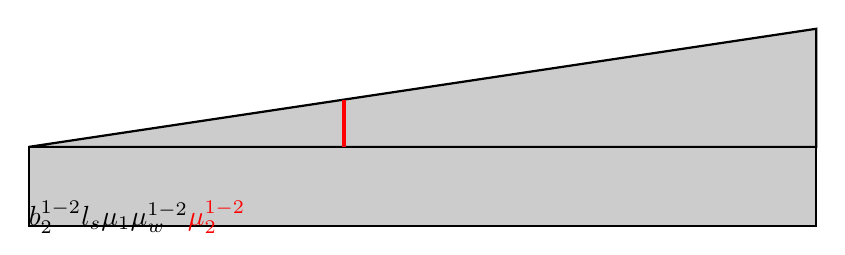
\begin{tikzpicture}
\draw[fill=black!20,thick] (0,0) rectangle (10,1);
\draw[fill=black!20,thick] (0,1) -- (10,1) -- (10,2.5) -- cycle;
\draw[red,ultra thick] (4,1) -- (4,1.6);
\dimensioning{1}{4,0}{10,0}{-.7}[$b_2^{1-2}$];
\dimensioning{1}{0,0}{10,0}{-1.4}[$l_s$];
\dimensioning{2}{10,0}{10,1}{10.7}[$\mu_1$];
\dimensioning{2}{10,0}{10,2.5}{11.4}[$\mu_w^{1-2}$];
\begin{scope}[color=red]
\dimensioning{2}{10,0}{10,1.6}{12.1}[$\mu_2^{1-2}$];
\end{scope}
\end{tikzpicture}
\caption{Coefficiente $\mu_2$ calcolato tramite somma dell'altezza del triangolo (ottenuta per similitudine rispetto la base) e il coefficiente $\mu_1$}
\label{fig:TriangoliSimiliNeve}
\end{figure}
Usando la similitudine dei triangoli come mostrato in figura \ref{fig:TriangoliSimiliNeve} si ottiene l'altezza del triangolo a distanza $b_2$ dall'edificio e che sommato al valore dell'altezza $\mu_1$ del rettangolo porta al valore del \normaref{caso 2} cercato 
\begin{align*}
	\mu_2^{1}=&\mu_1 + \frac{(l_s - b_2^1)\cdot (\mu_w^1-\mu_1)}{l_s} = 1.386\\
	\mu_2^{2}=&\mu_1 + \frac{(l_s - b_2^2)\cdot (\mu_w^2-\mu_1)}{l_s} =	1.470
\end{align*}
Per semplicità si assume ora un valore unico del coefficiente tra i valori delle altezze del trapezio del caso 2 e pari alla media tra $\mu_2$ e $\mu_w$ ottenendo $\mu^1= 1.661$ e $\mu^2=1.602$ e costante.

Il carico dovuto alla neve sul terrazzo risulta infine pari a 
\begin{align}
q_s^1 &= q_{sk} \cdot C_E \cdot C_t \cdot \mu^1 = \SI{1.626}{} \cdot 1 \cdot 1 \cdot 1.661 = \SI{2.700}{\kilo\newton\per\square\meter}\\
q_s^2 &= q_{sk} \cdot C_E \cdot C_t \cdot \mu^2 = \SI{1.626}{} \cdot 1 \cdot 1 \cdot 1.602 = \SI{2.605}{\kilo\newton\per\square\meter}\label{eq:qneve}
\end{align}
\paragraph*{Vento} \label{cap:ventoTerrazzo} 
La velocità base di riferimento $V_b$ è data dalla \normaref{3.3.1} delle \norma{NTC2018} e dalla relativa \normaref{Tab.\,3.3.1} nel quale il coefficiente di altitudine $c_a$ vale $1$ perché la quota è inferiorie ad $a_0$ e $V_{b,o}=\SI{25}{\meter\per\second}$. 
Il coefficiente di ritorno $c_r$ della \normaref{Formula\,3.3.2} è pari a $1$ nel caso di un tempo pari a 50 anni. 
Pertanto la velocità di riferimento $V_r=\SI{25}{\meter\per\second}$.
Assumendo una densità dell'aria $\rho$ come consigliato nel \normaref{\S\,3.3.6}, la pressione cinetica di riferimento vale $q_r =1/2\, \rho\, V_r^2 = \SI{0.39}{\kilo\newton\per\square\meter}$. 

L'edificio è ubicato in provincia di Trento pertanto è in zona urbana ad una quota inferiore a \SI{500}{\meter} ed ad una distanza maggiore di \SI{30}{\kilo\meter} dal mare. 
Risulta quindi dalla \normaref{Tab.\,3.3.III} una classe di rugosità del terreno A e dalla \normaref{Fig.\,3.3.2} una classe di esposizione V del sito.
Pertanto dalla \normaref{Tab.\,3.3.II} si ha
\[
	k_r=0.23 \qquad z_0=\SI{0.70}{\meter} \quad z_{min}=\SI{12}{\meter}
\]
Il coefficiente di topografia $c_t$ è assunto pari a $1$.
La quota del terrazzo in cui si sta calcolando l'azione del vento è pari a \SI{3.50}{\meter}.
Il coefficiente di esposizione risulta pari alla \normaref{Formula\,3.3.7} 
\[
	c_e(z)=c_e(z_{min})=k_t^2\cdot c_t \cdot \ln(z/z_0)\cdot[7+c_t\cdot\ln (z/z_0)] = 1.48
\]

Per il calcolo del coefficiente di pressione $c_p$ si è preso come riferimento il \normaref{\S\,C3.3.8.1.2} riguardante le coperture piane non essendo elencati nelle normative casi specifici per i terrazzi.

Si sono utilizzati i coefficienti globali in quanto si vuole calcolare la pressione o depressione complessiva esercitata dalla forza del vento. 
Si avranno due valori di pressione positivi e negativi e che verranno usati per ottenere poi (nel paragrafo \ref{cap:combinazioniCarico}) i valori sfavorevoli e favorevoli.

\begin{figure*}[htbp]
\centering
\includegraphics{IMG/figC3-3-5.pdf}
\label{fig:C335}
\end{figure*}
Per il calcolo del coefficiente $C_{pe}$ la \norma{circolare} in \normaref{Fig.\,C.3.3.5} e \normaref{Tab.\,C.3.3.III} propone la distinzione di due zone A e B, la prima avente dimensione $\min\{ b/2\,;\,h\}$ che nel caso in esame è pari a $\min\{\frac{\SI{33.65}{\meter}}{2};\SI{3.50}{\meter}\}=\SI{3.50}{\meter}$.
Essendo quindi il terrazzo delimitato da entrambe le zone e non volendo calcolare la forza totale del vento ma il carico su superficie, si è considerato nel caso di pressione il coefficiente positivo $C_{pe,B}=+0.2$ da usare nel caso sfavorevole e il coefficiente negativo $C_{pe,B}=-0.20$ da usare nel caso favorevole di depressione.
Quest'ultimo in realtà a favore di sicurezza in quanto sarebbe da considerare anche il coefficiente $C_{pe,A}=-0.80$.

Il coefficiente dinamico $c_d$ è preso pari ad 1 come suggerito nel capitolo \normaref{\S\,3.3.9}

Pertanto il carico dovuto al vento è pari a 
\begin{equation}
	q_w = q_r \cdot c_e \cdot c_p \cdot c_d = \SI{0.39}{\kilo\newton\per\square\meter}\cdot 1.48 \cdot \pm 0.20 \cdot 1= \pm \SI{0.1154}{\kilo\newton\per\square\meter}\label{eq:caricoVento}
\end{equation}
\subsection{Interno}
\paragraph*{Carichi permanenti strutturali G1}
\e presente il medesimo solaio strutturale del terrazzo, pertanto $g_1^{sol.}=\SI{3.20}{\kilo\newton\per\square\meter}$.
\paragraph*{Carichi permanenti non strutturali G2}\label{cap:g2Trave} Sono costituiti dal pacchetto non strutturale della stratigrafia del solaio e dalle pareti divisorie interne. 
Per quanto riguarda le pareti divisorie interne il \normaref{\S\,3.1.3} delle \norma{NTC2018} permette di spalmare il peso delle pareti interne in un carico distribuito su tutta la superficie.
\begin{center}
\begin{tabular}{lS[table-format=2.1]S[table-format=1.2]S[table-format=1.3]}
	\toprule
	\multirow{2}{*}{Strato} & \multicolumn{1}{c}{Peso specifico} & \multicolumn{1}{c}{Spessore}& \multicolumn{1}{c}{$g_{2,k}$}\\
    	   & \multicolumn{1}{c}{$\left[\SI{}{\kilo\newton\per\meter\cubed}\right]$} & \multicolumn{1}{c}{$\left[\SI{}{\meter}\right]$}& \multicolumn{1}{c}{$\left[\SI{}{\kilo\newton\per\square\meter}\right]$}\\
	\midrule
	Tramezze in laterizio 	 	 & 8.00 & 0.08 & 0.64 \\
	Intonaco interno 	     	 & 20.0 & 0.01 & 0.2 \\
	Intonaco esterno	         & 20.0 & 0.01 & 0.2 \\
	\midrule
	Totale $=$   				 &      &      & 1.04 \\
	\bottomrule
\end{tabular}
\end{center}
L'altezza delle pareti corrisponde all'altezza di interpiano meno lo spessore del solaio, il che risulta $\SI{3.10}{} - \SI{0.25}{} = \SI{2.85}{\meter}$.
Il carico lineare delle pareti interne diviene quindi \SI{2.964}{\kilo\newton\per\meter}.
Utilizzando la normativa si ottiene così un carico di \SI{1.20}{\kilo\newton\per\square\meter}.

Unendo tutti i contributi si ha 
\begin{center}
\begin{tabular}{lS[table-format=2.1]S[table-format=1.2]S[table-format=1.3]}
	\toprule
	\multirow{2}{*}{Strato} & \multicolumn{1}{c}{Peso specifico} & \multicolumn{1}{c}{Spessore}& \multicolumn{1}{c}{$g_{2,k}$}\\
    	   & \multicolumn{1}{c}{$\left[\SI{}{\kilo\newton\per\meter\cubed}\right]$} & \multicolumn{1}{c}{$\left[\SI{}{\meter}\right]$}& \multicolumn{1}{c}{$\left[\SI{}{\kilo\newton\per\square\meter}\right]$}\\
	\midrule
	Sottofondo CLS alleggerito 	 & 16.0 & 0.08 & 1.28 \\
	Massetto allettamento 	     & 24.0 & 0.06 & 1.44 \\
	Pavimento ceramica 	         &      &      & 0.50 \\
	Intonaco intradosso 	     & 20.0 & 0.01 & 0.20 \\
	Pareti interne distribuite   &      &      & 1.20 \\
	\midrule
	Totale $g_2^{sol.} =$        &      &      & 4.62 \\
	\bottomrule
\end{tabular}
\end{center}
\paragraph*{Categoria B - Uffici} La \normaref{Tab.\,3.1.II} prevede un carico variabile di \SI{3.00}{\kilo\newton\per\square\meter} per la categoria uffici.
\subsection{Pareti perimetrali}\label{cap:paretiPerimetrali}
Sono agenti direttamente con un carico lineare al di sopra della trave e si estendono per una altezza pari a quella di interpiano meno la trave.
Ovvero $\SI{3.10}{} - \SI{0.5}{} = \SI{2.60}{\meter}$.
\begin{center}
\begin{tabular}{lS[table-format=2.1]S[table-format=1.2]S[table-format=1.3]}
	\toprule
	\multirow{2}{*}{Strato} & \multicolumn{1}{c}{Peso specifico} & \multicolumn{1}{c}{Spessore}& \multicolumn{1}{c}{$g_{2,k}$}\\
    	   & \multicolumn{1}{c}{$\left[\SI{}{\kilo\newton\per\meter\cubed}\right]$} & \multicolumn{1}{c}{$\left[\SI{}{\meter}\right]$}& \multicolumn{1}{c}{$\left[\SI{}{\kilo\newton\per\square\meter}\right]$}\\
	\midrule
	Muratura in laterizio 	 	 & 10   & 0.30 & 3 \\
	Intonaco interno 	     	 & 20.0 & 0.01 & 0.2 \\
	Cappotto esterno	         & 0.20 & 0.12 & 0.024 \\
	\midrule
	Totale $=$   				 &      &      & 3.224 \\
	\bottomrule
\end{tabular}
\end{center}
\begin{equation}
G_2^{pareti}=\SI{3.224}{\kilo\newton\per\square\meter} \cdot \SI{2.60}{\meter} = \SI{8.382}{\kilo\newton\per\meter}
\label{eq:paretiPerimetrali}
\end{equation}
\section{Totale carichi agenti sulla trave}
Vengono ora moltiplicati i risultati appena trovati per le relative lunghezze di influenza. 
Si è diviso il problema in tre zone: A, B e C come mostrato in figura \ref{fig:traveZonaABC}. 
\begin{figure}[tbp]
\centering
\includegraphics[trim=5.8cm 13cm 9.5cm 4.1cm,clip,frame,width=\textwidth]{IMG/Piante/Piante-ABC.pdf} 
\caption{Suddivisione del terrazzo in base alle tre diverse lunghezze di influenza.}
\label{fig:traveZonaABC}
\end{figure}
Nella zona A e B si ha una zona esterna dell'edificio e una zona interna.
Pertanto si considera il carico gravante sulla trave in oggetto di calcolo spalmato sui $5/8$ della luce nella zona verso l'esterno e alla metà della luce nella zona sottostante.  
Diviene rispettivamente pari a 
\begin{align*}
	\text{A :}&\qquad L^{ter.}=\frac{5}{8}\cdot\SI{6.00}{\meter}=\SI{3.75}{\meter} \qquad 
				L^{sol.} \frac{1}{2}\cdot\SI{5.00}{\meter} = \SI{2.50}{\meter}\\
	\text{B :}&\qquad L^{ter.}=\frac{5}{8}\cdot\SI{3.50}{\meter}=\SI{2.19}{\meter} \qquad 
				L^{sol.} \frac{1}{2}\cdot\SI{5.00}{\meter} = \SI{2.50}{\meter}\\
\end{align*}
Nella zona C invece l'orditura del solaio del terrazzo al primo piano è nell'altra direzioni. 
A tal proposito si considera una lunghezza di influenza del terrazzo simbolica di \SI{1.00}{\meter}.
Nella parte sottostante è uguale a quella delle altre zone.
\[
	\text{C :}\qquad L^{ter.}=\SI{1.00}{\meter} \qquad 
				L^{sol.} \frac{1}{2}\cdot\SI{5.00}{\meter} = \SI{2.50}{\meter}
\]

I carichi a metro lineare sotto riportati tenendo conto di tali lunghezze e sono stati combinati con le relativi azioni agenti sulla trave.

Nel caso dei sovraccarichi variabili si è assunta l'ipotesi che essi agiscano sempre insieme. 
Ovvero quando è possibile che avvenga il valore caratteristico nel terrazzo, questo avverrà anche nel solaio interno.
\paragraph*{Zona A} 
\[
\begin{split}
G_1^A &=  g_1^{ter.}\cdot L^{ter.} + g_1^{sol.}\cdot L^{sol.} + G_1^{trave} \\
&= \SI{3.20}{\kilo\newton\per\square\meter}\cdot\SI{3.75}{\meter} + \SI{3.20}{\kilo\newton\per\square\meter}\cdot\SI{2.50}{\meter} + \SI{3.75}{\kilo\newton\per\meter} \\
&= \SI{23.75}{\kilo\newton\per\meter} \\
G_2^A &= g_2^{ter.}\cdot L^{ter.} + g_2^{sol.}\cdot L^{sol.} + G_2^{pareti} \\
&= \SI{2.215}{\kilo\newton\per\square\meter}\cdot\SI{3.75}{\meter} + \SI{4.62}{\kilo\newton\per\square\meter}\cdot\SI{2.50}{\meter} + \SI{8.382}{\kilo\newton\per\meter} \\
&= \SI{28.24}{\kilo\newton\per\meter}\\
Q_{cat. B}^A &= q_{cat. B}^{ter.}\cdot L^{ter.} + q_{cat. B}^{sol.}\cdot L^{sol.} \\
&= \SI{4.00}{\kilo\newton\per\square\meter}\cdot\SI{3.75}{\meter} + \SI{3.00}{\kilo\newton\per\square\meter}\cdot\SI{2.50}{\meter} \\
&= \SI{22.50}{\kilo\newton\per\meter}\\
Q_{neve}^A &= q_s \cdot L^{ter.} = \SI{2.700}{\kilo\newton\per\square\meter}\cdot\SI{3.75}{\meter} = \SI{10.13}{\kilo\newton\per\meter}\\
Q_{vento}^A &= q_w \cdot L^{ter.} = \SI{\pm 0.1154}{\kilo\newton\per\square\meter}\cdot\SI{3.75}{\meter} = \SI{\pm 0.4328}{\kilo\newton\per\meter}
\end{split}
\]
\paragraph*{Zona B} I carichi su superficie sono gli stessi della zona A ma cambiano le lunghezze di riferimento e il carico della neve $q_s$ come visto nella \eqref{eq:qneve}. 
Si ha perciò
\begin{align*}
G_1^B &= \SI{18.76}{\kilo\newton\per\meter}\\
G_2^B &= \SI{24.78}{\kilo\newton\per\meter}\\
Q_{cat. B}^B &=  \SI{16.26}{\kilo\newton\per\meter}\\
Q_{neve}^B &= \SI{5.705}{\kilo\newton\per\meter}\\
Q_{vento}^B &= \SI{\pm 0.2527}{\kilo\newton\per\meter}
\end{align*}
\paragraph*{Zona C} Si hanno gli stessi carichi della zona A con la relativa lunghezza di riferimento
\begin{align*}
G_1^C &= \SI{14.95}{\kilo\newton\per\meter}\\
G_2^C &= \SI{22.15}{\kilo\newton\per\meter}\\
Q_{cat. B}^C &=  \SI{11.50}{\kilo\newton\per\meter}\\
Q_{neve}^C &= \SI{2.700}{\kilo\newton\per\meter}\\
Q_{vento}^C &= \SI{\pm 0.1554}{\kilo\newton\per\meter}
\end{align*}
\section{Combinazioni di carico}\label{cap:combinazioniCarico}
Al fine di trovare le azioni più incisive nel caso di carico massimo e di carico minimo, si sono valutate le azioni sfavorevoli e favorevoli con diverse disposizione nelle campate. 
Si elencheranno qui le diverse possibili combinazioni di carico agli stati limite ultimi e di esercizio.
\paragraph*{Zona A}
\allowdisplaybreaks %Serve per fare andare le equazioni su più pagine. Non spezza gli split perché non hanno questa possibilità (meglio). Per spezzare in un punto specifico \displaybreak
\begin{align} 
	\begin{split}
	SLU^{\text{sfav}}_{\text{cat. B}} &= \gamma_{G1}\cdot G_1 + \gamma_{G2} \cdot G_2 + \gamma_{cat. B} \cdot Q_{cat. B} + \gamma_{neve}\cdot Q_{neve}\cdot\psi_{02} + \gamma_{vento}\cdot Q_{vento} \cdot \psi_{03}  \\
	&= 1.3\cdot\SI{23.75}{} + 1.5\cdot\SI{28.24}{} + 1.5\cdot\SI{22.50}{} + 1.5\cdot\SI{10.13}{}\cdot0.5 + 1.5\cdot\SI{0.4328}{}\cdot0.6\\
	&= \SI{115.0}{\kilo\newton\per\meter}
	\end{split} \\ 
	\begin{split}
	SLU^{\text{sfav}}_{\text{neve}} &= \gamma_{G1}\cdot G_1 + \gamma_{G2} \cdot G_2 + \gamma_{neve}\cdot Q_{neve} + \gamma_{cat. B} \cdot Q_{cat. B}\cdot\psi_{02} + \gamma_{vento}\cdot Q_{vento} \cdot \psi_{03}  \\
	&= 1.3\cdot\SI{23.75}{} + 1.5\cdot\SI{28.24}{} + 1.5\cdot\SI{10.13}{} + 1.5\cdot\SI{22.50}{}\cdot0.7 + 1.5\cdot\SI{0.4328}{}\cdot0.6\\
	&= \SI{112.4}{\kilo\newton\per\meter}
	\end{split} \\ 
	\begin{split}
	SLU^{\text{sfav}}_{\text{vento}} &= \gamma_{G1}\cdot G_1 + \gamma_{G2} \cdot G_2 + \gamma_{vento}\cdot Q_{vento} + \gamma_{cat. B} \cdot Q_{cat. B}\cdot\psi_{02} + \gamma_{neve}\cdot Q_{neve} \cdot \psi_{03}  \\
	&= 1.3\cdot\SI{23.75}{} + 1.5\cdot\SI{28.24}{} + 1.5\cdot\SI{0.4328}{} + 1.5\cdot\SI{22.50}{}\cdot0.7 + 1.5\cdot\SI{10.13}{}\cdot0.5\\
	&= \SI{105.1}{\kilo\newton\per\meter}
	\end{split} \\ 
	\begin{split}
	SLU^{\text{fav}} &= \gamma_{G1}\cdot G_1 + \gamma_{G2} \cdot G_2 + \varnothing\\
	&= 1.0\cdot\SI{23.75}{} + 0.8\cdot\SI{28.24}{}\\
	&= \SI{46.34}{\kilo\newton\per\meter}	
	\end{split} \\ 
	\begin{split}
	SLE^{\text{rara}}_{\text{cat. B}} &= G_1 + G_2 + Q_{cat. B} + \psi_{02}\cdot Q_{neve} + \psi_{03}\cdot Q_{vento}  \\
	&= \SI{23.75}{} + \SI{28.24}{} + \SI{22.50}{} + 0.5\cdot\SI{10.13}{} + 0.6\cdot\SI{0.4328}{}\\
	&= \SI{79.81}{\kilo\newton\per\meter}
	\end{split} \\ 
	\begin{split}
	SLE^{\text{rara}}_{\text{neve}} &= G_1 + G_2 + Q_{neve} + \psi_{02}\cdot Q_{cat. B} + \psi_{03}\cdot Q_{vento}  \\
	&= \SI{23.75}{} + \SI{28.24}{} + \SI{10.13}{} + 0.7\cdot\SI{22.50}{} + 0.6\cdot\SI{0.4328}{}\\
	&= \SI{78.13}{\kilo\newton\per\meter}
	\end{split} \\ 
	\begin{split}
	SLE^{\text{rara}}_{\text{vento}} &= G_1 + G_2 + Q_{vento} + \psi_{02}\cdot Q_{cat. B} + \psi_{03}\cdot Q_{neve}  \\
	&= \SI{23.75}{} + \SI{28.24}{} + \SI{0.4328}{} + 0.7\cdot\SI{22.50}{} + 0.6\cdot\SI{10.13}{}\\
	&= \SI{74.25}{\kilo\newton\per\meter}
	\end{split} \\ 
	\begin{split}
	SLE^{\text{frequente}}_{\text{cat. B}} &= G_1 + G_2 + \psi_{11}\cdot Q_{cat. B} + \psi_{22}\cdot Q_{neve} + \psi_{23}\cdot Q_{vento}  \\
	&= \SI{23.75}{} + \SI{28.24}{} + 0.5\cdot\SI{22.50}{} + \varnothing +\varnothing\\
	&= \SI{63.24}{\kilo\newton\per\meter}
	\end{split} \\ 
	\begin{split}
	SLE^{\text{frequente}}_{\text{neve}} &= G_1 + G_2 + \psi_{11}\cdot Q_{neve} + \psi_{22}\cdot Q_{cat. B} + \psi_{23}\cdot Q_{vento}  \\
	&= \SI{23.75}{} + \SI{28.24}{} + 0.2\cdot\SI{10.13}{} + 0.3\cdot\SI{22.50}{} + \varnothing \\
	&= \SI{60.77}{\kilo\newton\per\meter}
	\end{split} \\ 
	\begin{split}
	SLE^{\text{frequente}}_{\text{vento}} &= G_1 + G_2 + \psi_{11}\cdot Q_{vento} + \psi_{22}\cdot Q_{cat. B} + \psi_{23}\cdot Q_{neve}  \\
	&= \SI{23.75}{} + \SI{28.24}{} + 0.2\cdot\SI{0.4328}{} + 0.3\cdot\SI{22.50}{} + \varnothing\\
	&= \SI{58.83}{\kilo\newton\per\meter}
	\end{split} \\ 
	\begin{split}
	SLE^{\text{quasi perm.}}_{\text{cat. B}} &= G_1 + G_2 + \psi_{21}\cdot Q_{cat. B} + \psi_{22}\cdot Q_{neve} + \psi_{23}\cdot Q_{vento} \\
	&= \SI{23.75}{} + \SI{28.24}{} + 0.3\cdot\SI{22.50}{} + \varnothing + \varnothing \\
	&= \SI{58.74}{\kilo\newton\per\meter}
	\end{split} 
\end{align}
\paragraph*{Zona B} Analogamente
\begin{align*} 
	SLU^{\text{sfav}}_{\text{cat. B}}		&= \SI{90.23}{\kilo\newton\per\meter} \\
	SLU^{\text{sfav}}_{\text{neve}} 		&= \SI{87.42}{\kilo\newton\per\meter} \\
	SLU^{\text{sfav}}_{\text{vento}} 		&= \SI{83.29}{\kilo\newton\per\meter} \\
	SLU^{\text{fav}} 						&= \SI{38.58}{\kilo\newton\per\meter} \\	
	SLE^{\text{rara}}_{\text{cat. B}} 		&= \SI{62.80}{\kilo\newton\per\meter} \\
	SLE^{\text{rara}}_{\text{neve}}			&= \SI{60.78}{\kilo\newton\per\meter} \\
	SLE^{\text{rara}}_{\text{vento}} 		&= \SI{58.60}{\kilo\newton\per\meter} \\
	SLE^{\text{frequente}}_{\text{cat. B}} 	&= \SI{51.67}{\kilo\newton\per\meter} \\
	SLE^{\text{frequente}}_{\text{neve}} 	&= \SI{49.56}{\kilo\newton\per\meter} \\
	SLE^{\text{frequente}}_{\text{vento}} 	&= \SI{48.47}{\kilo\newton\per\meter} \\
	SLE^{\text{quasi perm.}}_{\text{cat. B}}&= \SI{48.42}{\kilo\newton\per\meter}
\end{align*}
%
\paragraph*{Zona C} Analogamente
\begin{align*} 
	SLU^{\text{sfav}}_{\text{cat. B}}		&= \SI{71.94}{\kilo\newton\per\meter} \\
	SLU^{\text{sfav}}_{\text{neve}} 		&= \SI{68.92}{\kilo\newton\per\meter} \\
	SLU^{\text{sfav}}_{\text{vento}} 		&= \SI{66.99}{\kilo\newton\per\meter} \\
	SLU^{\text{fav}} 						&= \SI{32.67}{\kilo\newton\per\meter} \\	
	SLE^{\text{rara}}_{\text{cat. B}} 		&= \SI{50.04}{\kilo\newton\per\meter} \\
	SLE^{\text{rara}}_{\text{neve}}			&= \SI{47.94}{\kilo\newton\per\meter} \\
	SLE^{\text{rara}}_{\text{vento}} 		&= \SI{46.93}{\kilo\newton\per\meter} \\
	SLE^{\text{frequente}}_{\text{cat. B}} 	&= \SI{42.85}{\kilo\newton\per\meter} \\
	SLE^{\text{frequente}}_{\text{neve}} 	&= \SI{41.09}{\kilo\newton\per\meter} \\
	SLE^{\text{frequente}}_{\text{vento}} 	&= \SI{40.58}{\kilo\newton\per\meter} \\
	SLE^{\text{quasi perm.}}_{\text{cat. B}}&= \SI{40.55}{\kilo\newton\per\meter}
\end{align*}

\section{Risoluzione della trave mediante metodo delle forze}
Essendo la struttura composta da travi continue è stato adottato il metodo delle forze per la sua risoluzione, il quale risulta essere estremamente comodo in queste tipologie di strutture iperstatiche.
La struttura originaria iperstatica viene degradata ad un sistema di travi isostatico equivalente mediante l'inserimento di incognite iperstatiche, che nel caso di travi continue sono tutte di tipo rotazionale.

Si tratta quindi di imporre l'uguaglianza delle rotazioni tra una trave e l'altra e di risolvere l'equazione di congruenza trovando i termini incogniti.
In termini matriciali si ha il seguente sistema da risolvere:
\begin{equation}
\mathbf{Flex}\cdot\mathbf{A} =  \mathbf{P}.
\end{equation}

Per un generico sistema di trave continua a $6$ campate la matrice di flessibilità assume la forma
\begin{equation}
\mathbf{Flex^{gen}}=
\begin{bmatrix}
\frac{L_{1}}{3 \, \mathit{EJ}} & \frac{L_{1}}{6 \, \mathit{EJ}} & 0 & 0 & 0 & 0 & 0 \\
\frac{L_{1}}{6 \, \mathit{EJ}} & \frac{L_{1} + L_{2}}{3 \, \mathit{EJ}} & \frac{L_{2}}{6 \, \mathit{EJ}} & 0 & 0 & 0 & 0 \\
0 & \frac{L_{2}}{6 \, \mathit{EJ}} & \frac{L_{2} + L_{3}}{3 \, \mathit{EJ}} & \frac{L_{3}}{6 \, \mathit{EJ}} & 0 & 0 & 0 \\
0 & 0 & \frac{L_{3}}{6 \, \mathit{EJ}} & \frac{L_{3} + L_{4}}{3 \, \mathit{EJ}} & \frac{L_{4}}{6 \, \mathit{EJ}} & 0 & 0 \\
0 & 0 & 0 & \frac{L_{4}}{6 \, \mathit{EJ}} & \frac{L_{4} + L_{5}}{3 \, \mathit{EJ}} & \frac{L_{5}}{6 \, \mathit{EJ}} & 0 \\
0 & 0 & 0 & 0 & \frac{L_{5}}{6 \, \mathit{EJ}} & \frac{L_{5} + L_{6}}{3 \, \mathit{EJ}} & \frac{L_{6}}{6 \, \mathit{EJ}} \\
0 & 0 & 0 & 0 & 0 & \frac{L_{6}}{6 \, \mathit{EJ}} & \frac{L_{6}}{3 \, \mathit{EJ}}
\end{bmatrix}
\end{equation}
avendo però a sinistra l'appoggio e non l'incastro; va eliminata la prima riga e la prima colonna in quanto il momento è nullo.
Si ottiene perciò la matrice ridotta
\begin{equation}
\mathbf{Flex^{rid}}=
\begin{bmatrix}
\frac{L_{1} + L_{2}}{3 \, \mathit{EJ}} & \frac{L_{2}}{6 \, \mathit{EJ}} & 0 & 0 & 0 & 0 \\
\frac{L_{2}}{6 \, \mathit{EJ}} & \frac{L_{2} + L_{3}}{3 \, \mathit{EJ}} & \frac{L_{3}}{6 \, \mathit{EJ}} & 0 & 0 & 0 \\
0 & \frac{L_{3}}{6 \, \mathit{EJ}} & \frac{L_{3} + L_{4}}{3 \, \mathit{EJ}} & \frac{L_{4}}{6 \, \mathit{EJ}} & 0 & 0 \\
0 & 0 & \frac{L_{4}}{6 \, \mathit{EJ}} & \frac{L_{4} + L_{5}}{3 \, \mathit{EJ}} & \frac{L_{5}}{6 \, \mathit{EJ}} & 0 \\
0 & 0 & 0 & \frac{L_{5}}{6 \, \mathit{EJ}} & \frac{L_{5} + L_{6}}{3 \, \mathit{EJ}} & \frac{L_{6}}{6 \, \mathit{EJ}} \\
0 & 0 & 0 & 0 & \frac{L_{6}}{6 \, \mathit{EJ}} & \frac{L_{6}}{3 \, \mathit{EJ}}
\end{bmatrix}
\end{equation}
in cui sostituendo le grandezze in gioco diviene
\begin{equation}
\mathbf{F}=
\begin{bmatrix}
0.0000254 & 7.62 \times 10^{-6} & 0.000 & 0.000 & 0.000 & 0.000 \\
7.62 \times 10^{-6} & 0.0000288 & 6.78 \times 10^{-6} & 0.000 & 0.000 & 0.000 \\
0.000 & 6.78 \times 10^{-6} & 0.0000305 & 8.47 \times 10^{-6} & 0.000 & 0.000 \\
0.000 & 0.000 & 8.47 \times 10^{-6} & 0.0000378 & 0.0000104 & 0.000 \\
0.000 & 0.000 & 0.000 & 0.0000104 & 0.0000344 & 6.78 \times 10^{-6} \\
0.000 & 0.000 & 0.000 & 0.000 & 6.78 \times 10^{-6} & 0.0000136
\end{bmatrix}
\end{equation}.

Il generico vettore dei carichi per una struttura a 6 campate è
\begin{equation}
\mathbf{p^{gen}}=
\begin{bmatrix}
\frac{L_{1}^{3} Q_{1}}{24 \, \mathit{EJ}} \\
\frac{L_{1}^{3} Q_{1} + L_{2}^{3} Q_{2}}{24 \, \mathit{EJ}} \\
\frac{L_{2}^{3} Q_{2} + L_{3}^{3} Q_{3}}{24 \, \mathit{EJ}} \\
\frac{L_{3}^{3} Q_{3} + L_{4}^{3} Q_{4}}{24 \, \mathit{EJ}} \\
\frac{L_{4}^{3} Q_{4} + L_{5}^{3} Q_{5}}{24 \, \mathit{EJ}} \\
\frac{L_{5}^{3} Q_{5} + L_{6}^{3} Q_{6}}{24 \, \mathit{EJ}} \\
\frac{L_{6}^{3} Q_{6}}{24 \, \mathit{EJ}}
\end{bmatrix}
\end{equation}
a cui anche qui va adattato al caso senza incastro, divenendo
\begin{equation}
\mathbf{p^{rid}}=
\begin{bmatrix}
\frac{L_{1}^{3} Q_{1} + L_{2}^{3} Q_{2}}{24 \, \mathit{EJ}} \\
\frac{L_{2}^{3} Q_{2} + L_{3}^{3} Q_{3}}{24 \, \mathit{EJ}} \\
\frac{L_{3}^{3} Q_{3} + L_{4}^{3} Q_{4}}{24 \, \mathit{EJ}} \\
\frac{L_{4}^{3} Q_{4} + L_{5}^{3} Q_{5}}{24 \, \mathit{EJ}} \\
\frac{L_{5}^{3} Q_{5} + L_{6}^{3} Q_{6}}{24 \, \mathit{EJ}} \\
\frac{L_{6}^{3} Q_{6}}{24 \, \mathit{EJ}}
\end{bmatrix}
\end{equation}

%!TEX root = ../RelazioneStrutturaleMeoliNicola.tex
\begin{figure}[htb]
\centering
\begin{tikzpicture}
\scaling{0.55};
	\point{n1}{00.00}{0};
	\point{n2}{03.00}{0};
	\point{n3}{07.50}{0};
	\point{n4}{11.50}{0};
	\point{n5}{16.50}{0};
	\point{n6}{22.65}{0};
	\point{n7}{26.65}{0};
	\beam{2}{n1}{n2}[0][1];
	\beam{2}{n2}{n3}[1][1];
	\beam{2}{n3}{n4}[1][1];
	\beam{2}{n4}{n5}[1][1];
	\beam{2}{n5}{n6}[1][1];
	\beam{2}{n6}{n7}[1][1];
	\begin{scope}[scale=0.6]
		\support{1}{n1};
		\support{1}{n2};
		\support{1}{n3};
		\support{1}{n4};
		\support{1}{n5};
		\support{1}{n6};
		\support{3}{n7}[90];
	\end{scope};	
	\begin{scope}[color=myGray]
		\lineload{1}{n1}{n2};	
		\notation{1}{n2}{$Q_1=1$}[above=13mm];
	\end{scope}	
	\begin{scope}[color=red]
		\load{2}{n1}[280][130][0.70];
		\load{3}{n2}[130][130][0.70];
		\load{2}{n2}[280][130][0.70];
		\load{3}{n3}[130][130][0.70];
		\load{2}{n3}[280][130][0.70];
		\load{3}{n4}[130][130][0.70];
		\load{2}{n4}[280][130][0.70];
		\load{3}{n5}[130][130][0.70];
		\load{2}{n5}[280][130][0.70];
		\load{3}{n6}[130][130][0.70];
		\load{2}{n6}[280][130][0.70];
		\load{3}{n7}[130][130][0.70];
		\notation{1}{n1}{$x_{11}$}[below=8mm];
		\notation{1}{n2}{$x_{21}$}[below=8mm];
		\notation{1}{n3}{$x_{31}$}[below=8mm];
		\notation{1}{n4}{$x_{41}$}[below=8mm];
		\notation{1}{n5}{$x_{51}$}[below=8mm];
		\notation{1}{n6}{$x_{61}$}[below=8mm];
		\notation{1}{n7}{$x_{71}$}[below=8mm];
	\end{scope}
	\dimensioning{1}{n1}{n2}{-1.5}[$\SI{3.00}{\meter}$];
\end{tikzpicture}
\caption{Metodo delle forze applicato alla prima campata con carico unitario}
\label{fig:Struttura1}
\end{figure} 
Per trovare i vettori incognita va risolto il sistema i-esimo ponendo $1$ al carico nella i-esima campata e zero nelle altre.
Nel caso della prima si ha la situazione visibile in figura \ref{fig:Struttura1} in cui si sono riportati i momenti generatosi dal carico unitario nella prima campata.
Risolvendo il sistema si ha 
\begin{equation}
\mathbf{F\cdot x_1 = P^{rid}_{1}}
\end{equation}
\begin{equation}
\hookrightarrow \, \mathbf{x_1}=
\begin{bmatrix}
x_{11}\\
x_{21}\\
x_{31}\\
x_{41}\\
x_{51}\\
x_{61}\\
x_{71}\\
\end{bmatrix} =
\begin{bmatrix}
0\\
-0.491338912574569 \\
0.137796375248564 \\
-0.0328783181600082 \\
0.00812484517717799 \\
-0.00273048075626473 \\
0.00136524037813237
\end{bmatrix}
\end{equation} 
al quale è stato re-inserito il primo termine zero per ottenere la dimensione del vettore globale.
Lo stesso procedimento lo si adotta per le altre campate ottenendo 7 vettori $x_i$.

\e ora possibile calcolare le reazioni vincolari in ogni nodo aventi la generica forma
\begin{equation}
r_{j,i}=\frac{x_{j+1,i}-x_{j,i}}{L_i}+Q_i\cdot\frac{L_i}{2}
\end{equation} dove $Q_i$ vale $1$ solo quando si sta considerando la campata in cui è agente il carico ($i=j$) altrimenti vale zero, mentre con $j$ si è indicato il numero del nodo.

Nel caso della prima campata si ha
\begin{equation}
\mathbf{r_1}=
\begin{bmatrix}
\frac{x_{2,1}-x_{1,1}}{L_1}+\frac{Q_1\cdot L_1}{2} \\
\frac{x_{3,1}-x_{2,1}}{L_2} \\
\frac{x_{4,1}-x_{3,1}}{L_3} \\
\frac{x_{5,1}-x_{4,1}}{L_4} \\
\frac{x_{6,1}-x_{5,1}}{L_5} \\
\frac{x_{7,1}-x_{6,1}}{L_6} \\
\end{bmatrix} =
\begin{bmatrix}
1.33622036247514 \\
0.139807841738474 \\
-0.0426686733521431 \\
0.00820063266743724 \\
-0.00176509364771426 \\
0.00102393028359927
\end{bmatrix}
\end{equation}

\e possibile ora creare delle funzioni a gradini che esistono solo nel tratto di campata considerato e che esplicano i valori delle rotazioni e delle reazioni vincolari a sinistra e destra di ogni nodo.
Unendo le funzioni di ciascuna campata si ottengono le due funzioni totali per il momento e il taglio.

Creando un grafico relativo alla prima campata si ottiene l'andamento visibile in figura \ref{fig:MomentiUnitariA} e in figura \ref{fig:TagliUnitariA}.
Eseguendo queste operazioni per le altre campate è possibile risolvere appieno la struttura e sommando i risultati per ciascuna di esse si ottiene l'andamento totale di figura \ref{fig:MomentiUnitariTOT} e \ref{fig:TagliUnitariTOT} che rappresenta la condizione di carico unitario in tutte le campate.
\begin{figure}[p]
\centering
\subfloat[][\emph{Campata 1\label{fig:MomentiUnitariA}}]{\includegraphics[width=0.45\textwidth]{../imgExportSage/M1_pUnitario.pdf}} \quad
\subfloat[][\emph{Campata 2}]{\includegraphics[width=0.45\textwidth]{../imgExportSage/M2_pUnitario}} \\
\subfloat[][\emph{Campata 3}]{\includegraphics[width=0.45\textwidth]{../imgExportSage/M3_pUnitario}} \quad
\subfloat[][\emph{Campata 4}]{\includegraphics[width=0.45\textwidth]{../imgExportSage/M4_pUnitario}} \\
\subfloat[][\emph{Campata 5}]{\includegraphics[width=0.45\textwidth]{../imgExportSage/M5_pUnitario.pdf}} \quad
\subfloat[][\emph{Campata 6}]{\includegraphics[width=0.45\textwidth]{../imgExportSage/M6_pUnitario}} \\
\subfloat[][\emph{Somma delle campate\label{fig:MomentiUnitariTOT}}]{\includegraphics[width=0.6\textwidth]{../imgExportSage/Mtot_pUnitario}}
\caption{Diagrammi del momento applicando di volta in volta un carico unitario nelle campate e la somma nel diagramma del momento unitario totale}
\label{fig:MomentiUnitari}
\end{figure}
\begin{figure}[p]
\centering
\subfloat[][\emph{Campata 1\label{fig:TagliUnitariA}}]{\includegraphics[width=0.45\textwidth]{../imgExportSage/T1_pUnitario.pdf}} \quad
\subfloat[][\emph{Campata 2}]{\includegraphics[width=0.45\textwidth]{../imgExportSage/T2_pUnitario}} \\
\subfloat[][\emph{Campata 3}]{\includegraphics[width=0.45\textwidth]{../imgExportSage/T3_pUnitario}} \quad
\subfloat[][\emph{Campata 4}]{\includegraphics[width=0.45\textwidth]{../imgExportSage/T4_pUnitario}} \\
\subfloat[][\emph{Campata 5}]{\includegraphics[width=0.45\textwidth]{../imgExportSage/T5_pUnitario.pdf}} \quad
\subfloat[][\emph{Campata 6}]{\includegraphics[width=0.45\textwidth]{../imgExportSage/T6_pUnitario}} \\
\subfloat[][\emph{Somma delle campate\label{fig:TagliUnitariTOT}}]{\includegraphics[width=0.6\textwidth]{../imgExportSage/Ttot_pUnitario}}
\caption{Diagrammi del taglio applicando di volta in volta un carico unitario nelle campate e la somma nel diagramma del taglio unitario totale}
\label{fig:TagliUnitari}
\end{figure}
\clearpage %Altrimenti c'era una pagina con 4 righe
\section{Massimizzazione delle sollecitazioni}
Per massimizzare le azioni di momento e taglio in tutti i punti voluti della trave occorre creare diverse situazioni di carico in modo da ottenere l'effetto massimo in campata o appoggio.
I carichi utilizzati sono quelli sfavorevoli e favorevoli visti in precedenza a pagina \pageref{cap:combinazioniCarico}, i quali sono stati moltiplicati alle funzioni di momento e taglio relative ai carichi unitari.
Le diverse  disposizioni dei carichi utilizzate sono visibili in figura \ref{fig:Struttura2} a pagina \pageref{fig:Struttura2}.
Nelle didascalie sono inoltre indicati gli effetti che ciascuna disposizione vuole riprodurre.
%!TEX root = ../RelazioneStrutturaleMeoliNicola.tex
\begin{figure}[htb]
\centering
\subfloat[][\emph{DA PENSARCI \label{fig:Struttura2a}}]
{
	\begin{tikzpicture}
	\scaling{0.55};
		\point{n1}{00.00}{0};
		\point{n2}{03.00}{0};
		\point{n3}{07.50}{0};
		\point{n4}{11.50}{0};
		\point{n5}{16.50}{0};
		\point{n6}{22.65}{0};
		\point{n7}{26.65}{0};
		\beam{2}{n1}{n2}[0][1];
		\beam{2}{n2}{n3}[1][1];
		\beam{2}{n3}{n4}[1][1];
		\beam{2}{n4}{n5}[1][1];
		\beam{2}{n5}{n6}[1][1];
		\beam{2}{n6}{n7}[1][1];
		\begin{scope}[scale=0.6]
			\support{1}{n1};
			\support{1}{n2};
			\support{1}{n3};
			\support{1}{n4};
			\support{1}{n5};
			\support{1}{n6};
			\support{3}{n7}[90];
		\end{scope};	
		%
		\begin{scope}[color=red]
			 \lineload{1}{n1}{n2}[1.3][1.3];
			%\lineload{1}{n2}{n3}[1.3][1.3];
			 \lineload{1}{n3}{n4}[1.3][1.3];
			%\lineload{1}{n4}{n5}[1.3][1.3];
			 \lineload{1}{n5}{n6}[1.3][1.3];
			%\lineload{1}{n6}{n7}[1.3][1.3];
		\end{scope};
		\begin{scope}[color=blue]
			%\lineload{1}{n1}{n2}[0.8][0.8];
			 \lineload{1}{n2}{n3}[0.8][0.8];
			%\lineload{1}{n3}{n4}[0.8][0.8];
			 \lineload{1}{n4}{n5}[0.8][0.8];
			%\lineload{1}{n5}{n6}[0.8][0.8];
			 \lineload{1}{n6}{n7}[0.8][0.8];
		\end{scope};
	\end{tikzpicture}
} \\
\subfloat[][\emph{DA PENSARCI \label{fig:Struttura2b}}]
{
	\begin{tikzpicture}
	\scaling{0.55};
		\point{n1}{00.00}{0};
		\point{n2}{03.00}{0};
		\point{n3}{07.50}{0};
		\point{n4}{11.50}{0};
		\point{n5}{16.50}{0};
		\point{n6}{22.65}{0};
		\point{n7}{26.65}{0};
		\beam{2}{n1}{n2}[0][1];
		\beam{2}{n2}{n3}[1][1];
		\beam{2}{n3}{n4}[1][1];
		\beam{2}{n4}{n5}[1][1];
		\beam{2}{n5}{n6}[1][1];
		\beam{2}{n6}{n7}[1][1];
		\begin{scope}[scale=0.6]
			\support{1}{n1};
			\support{1}{n2};
			\support{1}{n3};
			\support{1}{n4};
			\support{1}{n5};
			\support{1}{n6};
			\support{3}{n7}[90];
		\end{scope};	
		%
		\begin{scope}[color=red]
			%\lineload{1}{n1}{n2}[1.3][1.3];
			 \lineload{1}{n2}{n3}[1.3][1.3];
			%\lineload{1}{n3}{n4}[1.3][1.3];
			 \lineload{1}{n4}{n5}[1.3][1.3];
			%\lineload{1}{n5}{n6}[1.3][1.3];
			 \lineload{1}{n6}{n7}[1.3][1.3];
		\end{scope};
		\begin{scope}[color=blue]
			 \lineload{1}{n1}{n2}[0.8][0.8];
			%\lineload{1}{n2}{n3}[0.8][0.8];
			 \lineload{1}{n3}{n4}[0.8][0.8];
			%\lineload{1}{n4}{n5}[0.8][0.8];
			 \lineload{1}{n5}{n6}[0.8][0.8];
			%\lineload{1}{n6}{n7}[0.8][0.8];
		\end{scope};
	\end{tikzpicture}
} \\
\subfloat[][\emph{DA PENSARCI \label{fig:Struttura2c}}]
{
	\begin{tikzpicture}
	\scaling{0.55};
		\point{n1}{00.00}{0};
		\point{n2}{03.00}{0};
		\point{n3}{07.50}{0};
		\point{n4}{11.50}{0};
		\point{n5}{16.50}{0};
		\point{n6}{22.65}{0};
		\point{n7}{26.65}{0};
		\beam{2}{n1}{n2}[0][1];
		\beam{2}{n2}{n3}[1][1];
		\beam{2}{n3}{n4}[1][1];
		\beam{2}{n4}{n5}[1][1];
		\beam{2}{n5}{n6}[1][1];
		\beam{2}{n6}{n7}[1][1];
		\begin{scope}[scale=0.6]
			\support{1}{n1};
			\support{1}{n2};
			\support{1}{n3};
			\support{1}{n4};
			\support{1}{n5};
			\support{1}{n6};
			\support{3}{n7}[90];
		\end{scope};	
		%
		\begin{scope}[color=red]
			 \lineload{1}{n1}{n2}[1.3][1.3];
			 \lineload{1}{n2}{n3}[1.3][1.3];
			%\lineload{1}{n3}{n4}[1.3][1.3];
			 \lineload{1}{n4}{n5}[1.3][1.3];
			%\lineload{1}{n5}{n6}[1.3][1.3];
			 \lineload{1}{n6}{n7}[1.3][1.3];
		\end{scope};
		\begin{scope}[color=blue]
			%\lineload{1}{n1}{n2}[0.8][0.8];
			%\lineload{1}{n2}{n3}[0.8][0.8];
			 \lineload{1}{n3}{n4}[0.8][0.8];
			%\lineload{1}{n4}{n5}[0.8][0.8];
			 \lineload{1}{n5}{n6}[0.8][0.8];
			%\lineload{1}{n6}{n7}[0.8][0.8];
		\end{scope};
	\end{tikzpicture}
} \\
\subfloat[][\emph{DA PENSARCI \label{fig:Struttura2d}}]
{
	\begin{tikzpicture}
	\scaling{0.55};
		\point{n1}{00.00}{0};
		\point{n2}{03.00}{0};
		\point{n3}{07.50}{0};
		\point{n4}{11.50}{0};
		\point{n5}{16.50}{0};
		\point{n6}{22.65}{0};
		\point{n7}{26.65}{0};
		\beam{2}{n1}{n2}[0][1];
		\beam{2}{n2}{n3}[1][1];
		\beam{2}{n3}{n4}[1][1];
		\beam{2}{n4}{n5}[1][1];
		\beam{2}{n5}{n6}[1][1];
		\beam{2}{n6}{n7}[1][1];
		\begin{scope}[scale=0.6]
			\support{1}{n1};
			\support{1}{n2};
			\support{1}{n3};
			\support{1}{n4};
			\support{1}{n5};
			\support{1}{n6};
			\support{3}{n7}[90];
		\end{scope};	
		%
		\begin{scope}[color=red]
			%\lineload{1}{n1}{n2}[1.3][1.3];
			 \lineload{1}{n2}{n3}[1.3][1.3];
			 \lineload{1}{n3}{n4}[1.3][1.3];
			%\lineload{1}{n4}{n5}[1.3][1.3];
			 \lineload{1}{n5}{n6}[1.3][1.3];
			 %\lineload{1}{n6}{n7}[1.3][1.3];
		\end{scope};
		\begin{scope}[color=blue]
			\lineload{1}{n1}{n2}[0.8][0.8];
			%\lineload{1}{n2}{n3}[0.8][0.8];
			%\lineload{1}{n3}{n4}[0.8][0.8];
			\lineload{1}{n4}{n5}[0.8][0.8];
			%\lineload{1}{n5}{n6}[0.8][0.8];
			\lineload{1}{n6}{n7}[0.8][0.8];
		\end{scope};
	\end{tikzpicture}
} \\
\subfloat[][\emph{DA PENSARCI \label{fig:Struttura2e}}]
{
	\begin{tikzpicture}
	\scaling{0.55};
		\point{n1}{00.00}{0};
		\point{n2}{03.00}{0};
		\point{n3}{07.50}{0};
		\point{n4}{11.50}{0};
		\point{n5}{16.50}{0};
		\point{n6}{22.65}{0};
		\point{n7}{26.65}{0};
		\beam{2}{n1}{n2}[0][1];
		\beam{2}{n2}{n3}[1][1];
		\beam{2}{n3}{n4}[1][1];
		\beam{2}{n4}{n5}[1][1];
		\beam{2}{n5}{n6}[1][1];
		\beam{2}{n6}{n7}[1][1];
		\begin{scope}[scale=0.6]
			\support{1}{n1};
			\support{1}{n2};
			\support{1}{n3};
			\support{1}{n4};
			\support{1}{n5};
			\support{1}{n6};
			\support{3}{n7}[90];
		\end{scope};	
		%
		\begin{scope}[color=red]
			 \lineload{1}{n1}{n2}[1.3][1.3];
			%\lineload{1}{n2}{n3}[1.3][1.3];
			 \lineload{1}{n3}{n4}[1.3][1.3];
			 \lineload{1}{n4}{n5}[1.3][1.3];
			%\lineload{1}{n5}{n6}[1.3][1.3];
			 \lineload{1}{n6}{n7}[1.3][1.3];
		\end{scope};
		\begin{scope}[color=blue]
			%\lineload{1}{n1}{n2}[0.8][0.8];
			 \lineload{1}{n2}{n3}[0.8][0.8];
			%\lineload{1}{n3}{n4}[0.8][0.8];
			%\lineload{1}{n4}{n5}[0.8][0.8];
			 \lineload{1}{n5}{n6}[0.8][0.8];
			%\lineload{1}{n6}{n7}[0.8][0.8];
		\end{scope};
	\end{tikzpicture}
} \\
\subfloat[][\emph{DA PENSARCI \label{fig:Struttura2f}}]
{
	\begin{tikzpicture}
	\scaling{0.55};
		\point{n1}{00.00}{0};
		\point{n2}{03.00}{0};
		\point{n3}{07.50}{0};
		\point{n4}{11.50}{0};
		\point{n5}{16.50}{0};
		\point{n6}{22.65}{0};
		\point{n7}{26.65}{0};
		\beam{2}{n1}{n2}[0][1];
		\beam{2}{n2}{n3}[1][1];
		\beam{2}{n3}{n4}[1][1];
		\beam{2}{n4}{n5}[1][1];
		\beam{2}{n5}{n6}[1][1];
		\beam{2}{n6}{n7}[1][1];
		\begin{scope}[scale=0.6]
			\support{1}{n1};
			\support{1}{n2};
			\support{1}{n3};
			\support{1}{n4};
			\support{1}{n5};
			\support{1}{n6};
			\support{3}{n7}[90];
		\end{scope};	
		%
		\begin{scope}[color=red]
			%\lineload{1}{n1}{n2}[1.3][1.3];
			 \lineload{1}{n2}{n3}[1.3][1.3];
			%\lineload{1}{n3}{n4}[1.3][1.3];
			 \lineload{1}{n4}{n5}[1.3][1.3];
			 \lineload{1}{n5}{n6}[1.3][1.3];
			%\lineload{1}{n6}{n7}[1.3][1.3];
		\end{scope};
		\begin{scope}[color=blue]
			 \lineload{1}{n1}{n2}[0.8][0.8];
			%\lineload{1}{n2}{n3}[0.8][0.8];
			 \lineload{1}{n3}{n4}[0.8][0.8];
			%\lineload{1}{n4}{n5}[0.8][0.8];
			%\lineload{1}{n5}{n6}[0.8][0.8];
			 \lineload{1}{n6}{n7}[0.8][0.8];
		\end{scope};
	\end{tikzpicture}
} \\
\subfloat[][\emph{DA PENSARCI \label{fig:Struttura2g}}]
{
	\begin{tikzpicture}
	\scaling{0.55};
		\point{n1}{00.00}{0};
		\point{n2}{03.00}{0};
		\point{n3}{07.50}{0};
		\point{n4}{11.50}{0};
		\point{n5}{16.50}{0};
		\point{n6}{22.65}{0};
		\point{n7}{26.65}{0};
		\beam{2}{n1}{n2}[0][1];
		\beam{2}{n2}{n3}[1][1];
		\beam{2}{n3}{n4}[1][1];
		\beam{2}{n4}{n5}[1][1];
		\beam{2}{n5}{n6}[1][1];
		\beam{2}{n6}{n7}[1][1];
		\begin{scope}[scale=0.6]
			\support{1}{n1};
			\support{1}{n2};
			\support{1}{n3};
			\support{1}{n4};
			\support{1}{n5};
			\support{1}{n6};
			\support{3}{n7}[90];
		\end{scope};	
		%
		\begin{scope}[color=red]
			 \lineload{1}{n1}{n2}[1.3][1.3];
			%\lineload{1}{n2}{n3}[1.3][1.3];
			 \lineload{1}{n3}{n4}[1.3][1.3];
			%\lineload{1}{n4}{n5}[1.3][1.3];
			 \lineload{1}{n5}{n6}[1.3][1.3];
			 \lineload{1}{n6}{n7}[1.3][1.3];
		\end{scope};
		\begin{scope}[color=blue]
			%\lineload{1}{n1}{n2}[0.8][0.8];
			 \lineload{1}{n2}{n3}[0.8][0.8];
			%\lineload{1}{n3}{n4}[0.8][0.8];
			 \lineload{1}{n4}{n5}[0.8][0.8];
			%\lineload{1}{n5}{n6}[0.8][0.8];
			%\lineload{1}{n6}{n7}[0.8][0.8];
		\end{scope};
	\end{tikzpicture}
}
\caption{Disposizione dei carichi sfavorevoli e favorevoli}
\label{fig:Struttura2}
\end{figure}


Si ottiene così il diagramma finale cercato comprendente le azioni che la struttura di partenza genera.
In figura \ref{fig:Momenti_ULS} e successive è possibile visionare tali diagrammi per le 4 combinazioni SLU e SLE. 
A corredo dei diagrammi sono presenti inoltre delle tabelle che riassumono i valori più significativi.

Infine tra gli allegati della presente relazione, in particolare a pagina \pageref{cap:codiceTrave}, è inserito il codice scritto in \emph{SageMath} con il quale sono stati risolti i qui sopra visti passaggi.
%%%%%%%%%%%%%%%%%%%%%%%%%%%%%%%%%%%%%%%%%%%%%%%%%%%%%%%%%
\clearpage	
\begin{landscape}
\subsection*{SLU}
\begin{figure}[H]
\centering
\subfloat[][\emph{Sovrapposizione dei diagrammi del momento dovuta alle diverse casistiche di carico illustrate in figura \ref{fig:Struttura2} \label{fig:MomentiA_ULS}}]{\includegraphics[height=0.5\textwidth]{../imgExportSage/ULS_ptot.pdf}} 
\subfloat[][\emph{Inviluppo dei diagrammi del momento sovrapposti \label{fig:MomentiB_ULS}}]{\includegraphics[height=0.5\textwidth]{../imgExportSage/ULS_pInviluppo.pdf}} 
\caption{Diagrammi del momento generati con combinazione di carico SLU}
\label{fig:Momenti_ULS}
\end{figure}
\begin{table}[H]
\centering
\caption{Valori del momento con combinazione di carico SLU nei punti più significativi della struttura}
	\begin{tabular}{lS[table-format=3.2]S[table-format=3.2]S[table-format=3.2]S[table-format=3.2]S[table-format=3.2]S[table-format=3.2]S[table-format=3.2]S[table-format=3.2]S[table-format=3.2]S[table-format=3.2]S[table-format=3.2]S[table-format=3.2]S[table-format=3.2]}
		\toprule
		&\multicolumn{1}{c}{Nodo 1}&\multicolumn{1}{c}{Camp. 1}&\multicolumn{1}{c}{Nodo 2}&\multicolumn{1}{c}{Camp. 2}&\multicolumn{1}{c}{Nodo 3}&\multicolumn{1}{c}{Camp. 3}&\multicolumn{1}{c}{Nodo 4}&\multicolumn{1}{c}{Camp. 4}&\multicolumn{1}{c}{Nodo 5}&\multicolumn{1}{c}{Camp. 5}&\multicolumn{1}{c}{Nodo 6}&\multicolumn{1}{c}{Camp. 6}&\multicolumn{1}{c}{Nodo 7}\\
		\midrule
		$M^{-}$&999.99&999.99&999.99&999.99&999.99&999.99&999.99&999.99&999.99&999.99&999.99&999.99&999.99\\
		$M^{+}$&999.99&999.99&999.99&999.99&999.99&999.99&999.99&999.99&999.99&999.99&999.99&999.99&999.99\\
		\bottomrule
	\end{tabular}
\end{table}
\end{landscape}
\clearpage
\begin{landscape}
\subsection*{SLU}
\begin{figure}[H]
\centering
\subfloat[][\emph{Sovrapposizione dei diagrammi del taglio dovuta alle diverse casistiche di carico illustrate in figura \ref{fig:Struttura2} \label{fig:TagliA_ULS}}]{\includegraphics[height=0.5\textwidth]{../imgExportSage/ULS_Tptot.pdf}} 
\subfloat[][\emph{Inviluppo dei diagrammi del taglio sovrapposti \label{fig:TagliB_ULS}}]{\includegraphics[height=0.5\textwidth]{../imgExportSage/ULS_TpInviluppo.pdf}} 
\caption{Diagrammi del taglio generati con combinazione di carico SLU}
\label{fig:Tagli_ULS}
\end{figure}
\begin{table}[H]
\centering
\caption{Valori del taglio con combinazione di carico SLU nei punti più significativi della struttura}
	\begin{tabular}{lS[table-format=3.2]S[table-format=3.2]S[table-format=3.2]S[table-format=3.2]S[table-format=3.2]S[table-format=3.2]S[table-format=3.2]S[table-format=3.2]S[table-format=3.2]S[table-format=3.2]S[table-format=3.2]S[table-format=3.2]S[table-format=3.2]}
		\toprule
		&\multicolumn{1}{c}{Nodo 1}&\multicolumn{1}{c}{Camp. 1}&\multicolumn{1}{c}{Nodo 2}&\multicolumn{1}{c}{Camp. 2}&\multicolumn{1}{c}{Nodo 3}&\multicolumn{1}{c}{Camp. 3}&\multicolumn{1}{c}{Nodo 4}&\multicolumn{1}{c}{Camp. 4}&\multicolumn{1}{c}{Nodo 5}&\multicolumn{1}{c}{Camp. 5}&\multicolumn{1}{c}{Nodo 6}&\multicolumn{1}{c}{Camp. 6}&\multicolumn{1}{c}{Nodo 7}\\
		\midrule
		$M^{-}$&999.99&999.99&999.99&999.99&999.99&999.99&999.99&999.99&999.99&999.99&999.99&999.99&999.99\\
		$M^{+}$&999.99&999.99&999.99&999.99&999.99&999.99&999.99&999.99&999.99&999.99&999.99&999.99&999.99\\
		\bottomrule
	\end{tabular}
\end{table}
\end{landscape}
%%%%%%%%%%%%%%%%%%%%%%%%%%%%%%%%%%%%%%%%%%%%%%%%%%%%%%%%%
\clearpage	
\begin{landscape}
\subsection*{SLE -- Rara}
\begin{figure}[H]
\centering
\subfloat[][\emph{Sovrapposizione dei diagrammi del momento dovuta alle diverse casistiche di carico illustrate in figura \ref{fig:Struttura2} \label{fig:MomentiA_SLScharacteristic}}]{\includegraphics[height=0.5\textwidth]{../imgExportSage/SLScharacteristic_ptot.pdf}} 
\subfloat[][\emph{Inviluppo dei diagrammi del momento sovrapposti \label{fig:MomentiB_SLScharacteristic}}]{\includegraphics[height=0.5\textwidth]{../imgExportSage/SLScharacteristic_pInviluppo.pdf}} 
\caption{Diagrammi del momento generati con combinazione di carico SLE -- Rara}
\label{fig:Momenti_SLScharacteristic}
\end{figure}
\begin{table}[H]
\centering
\caption{Valori del momento con combinazione di carico SLE -- Rara nei punti più significativi della struttura}
	\begin{tabular}{lS[table-format=3.2]S[table-format=3.2]S[table-format=3.2]S[table-format=3.2]S[table-format=3.2]S[table-format=3.2]S[table-format=3.2]S[table-format=3.2]S[table-format=3.2]S[table-format=3.2]S[table-format=3.2]S[table-format=3.2]S[table-format=3.2]}
		\toprule
		&\multicolumn{1}{c}{Nodo 1}&\multicolumn{1}{c}{Camp. 1}&\multicolumn{1}{c}{Nodo 2}&\multicolumn{1}{c}{Camp. 2}&\multicolumn{1}{c}{Nodo 3}&\multicolumn{1}{c}{Camp. 3}&\multicolumn{1}{c}{Nodo 4}&\multicolumn{1}{c}{Camp. 4}&\multicolumn{1}{c}{Nodo 5}&\multicolumn{1}{c}{Camp. 5}&\multicolumn{1}{c}{Nodo 6}&\multicolumn{1}{c}{Camp. 6}&\multicolumn{1}{c}{Nodo 7}\\
		\midrule
		$M^{-}$&999.99&999.99&999.99&999.99&999.99&999.99&999.99&999.99&999.99&999.99&999.99&999.99&999.99\\
		$M^{+}$&999.99&999.99&999.99&999.99&999.99&999.99&999.99&999.99&999.99&999.99&999.99&999.99&999.99\\
		\bottomrule
	\end{tabular}
\end{table}
\end{landscape}
\clearpage
\begin{landscape}
\subsection*{SLE -- Rara}
\begin{figure}[H]
\centering
\subfloat[][\emph{Sovrapposizione dei diagrammi del taglio dovuta alle diverse casistiche di carico illustrate in figura \ref{fig:Struttura2} \label{fig:TagliA_SLScharacteristic}}]{\includegraphics[height=0.5\textwidth]{../imgExportSage/SLScharacteristic_Tptot.pdf}} 
\subfloat[][\emph{Inviluppo dei diagrammi del taglio sovrapposti \label{fig:TagliB_SLScharacteristic}}]{\includegraphics[height=0.5\textwidth]{../imgExportSage/SLScharacteristic_TpInviluppo.pdf}} 
\caption{Diagrammi del taglio generati con combinazione di carico SLU -- Rara}
\label{fig:Tagli_SLScharacteristic}
\end{figure}
\begin{table}[H]
\centering
\caption{Valori del taglio con combinazione di carico SLE -- Rara nei punti più significativi della struttura}
	\begin{tabular}{lS[table-format=3.2]S[table-format=3.2]S[table-format=3.2]S[table-format=3.2]S[table-format=3.2]S[table-format=3.2]S[table-format=3.2]S[table-format=3.2]S[table-format=3.2]S[table-format=3.2]S[table-format=3.2]S[table-format=3.2]S[table-format=3.2]}
		\toprule
		&\multicolumn{1}{c}{Nodo 1}&\multicolumn{1}{c}{Camp. 1}&\multicolumn{1}{c}{Nodo 2}&\multicolumn{1}{c}{Camp. 2}&\multicolumn{1}{c}{Nodo 3}&\multicolumn{1}{c}{Camp. 3}&\multicolumn{1}{c}{Nodo 4}&\multicolumn{1}{c}{Camp. 4}&\multicolumn{1}{c}{Nodo 5}&\multicolumn{1}{c}{Camp. 5}&\multicolumn{1}{c}{Nodo 6}&\multicolumn{1}{c}{Camp. 6}&\multicolumn{1}{c}{Nodo 7}\\
		\midrule
		$M^{-}$&999.99&999.99&999.99&999.99&999.99&999.99&999.99&999.99&999.99&999.99&999.99&999.99&999.99\\
		$M^{+}$&999.99&999.99&999.99&999.99&999.99&999.99&999.99&999.99&999.99&999.99&999.99&999.99&999.99\\
		\bottomrule
	\end{tabular}
\end{table}
\end{landscape}
%%%%%%%%%%%%%%%%%%%%%%%%%%%%%%%%%%%%%%%%%%%%%%%%%%%%%%%%%
\clearpage	
\begin{landscape}
\subsection*{SLE -- Frequente}
\begin{figure}[H]
\centering
\subfloat[][\emph{Sovrapposizione dei diagrammi del momento dovuta alle diverse casistiche di carico illustrate in figura \ref{fig:Struttura2} \label{fig:MomentiA_SLSfrequent}}]{\includegraphics[height=0.5\textwidth]{../imgExportSage/SLSfrequent_ptot.pdf}} 
\subfloat[][\emph{Inviluppo dei diagrammi del momento sovrapposti \label{fig:MomentiB_SLSfrequent}}]{\includegraphics[height=0.5\textwidth]{../imgExportSage/SLSfrequent_pInviluppo.pdf}} 
\caption{Diagrammi del momento generati con combinazione di carico SLE -- Frequente}
\label{fig:Momenti_SLSfrequent}
\end{figure}
\begin{table}[H]
\centering
\caption{Valori del momento con combinazione di carico SLE -- Frequente nei punti più significativi della struttura}
	\begin{tabular}{lS[table-format=3.2]S[table-format=3.2]S[table-format=3.2]S[table-format=3.2]S[table-format=3.2]S[table-format=3.2]S[table-format=3.2]S[table-format=3.2]S[table-format=3.2]S[table-format=3.2]S[table-format=3.2]S[table-format=3.2]S[table-format=3.2]}
		\toprule
		&\multicolumn{1}{c}{Nodo 1}&\multicolumn{1}{c}{Camp. 1}&\multicolumn{1}{c}{Nodo 2}&\multicolumn{1}{c}{Camp. 2}&\multicolumn{1}{c}{Nodo 3}&\multicolumn{1}{c}{Camp. 3}&\multicolumn{1}{c}{Nodo 4}&\multicolumn{1}{c}{Camp. 4}&\multicolumn{1}{c}{Nodo 5}&\multicolumn{1}{c}{Camp. 5}&\multicolumn{1}{c}{Nodo 6}&\multicolumn{1}{c}{Camp. 6}&\multicolumn{1}{c}{Nodo 7}\\
		\midrule
		$M^{-}$&999.99&999.99&999.99&999.99&999.99&999.99&999.99&999.99&999.99&999.99&999.99&999.99&999.99\\
		$M^{+}$&999.99&999.99&999.99&999.99&999.99&999.99&999.99&999.99&999.99&999.99&999.99&999.99&999.99\\
		\bottomrule
	\end{tabular}
\end{table}
\end{landscape}
\clearpage
\begin{landscape}
\subsection*{SLE -- Frequente}
\begin{figure}[H]
\centering
\subfloat[][\emph{Sovrapposizione dei diagrammi del taglio dovuta alle diverse casistiche di carico illustrate in figura \ref{fig:Struttura2} \label{fig:TagliA_SLSfrequent}}]{\includegraphics[height=0.5\textwidth]{../imgExportSage/SLSfrequent_Tptot.pdf}} 
\subfloat[][\emph{Inviluppo dei diagrammi del taglio sovrapposti \label{fig:TagliB_SLSfrequent}}]{\includegraphics[height=0.5\textwidth]{../imgExportSage/SLSfrequent_TpInviluppo.pdf}} 
\caption{Diagrammi del taglio generati con combinazione di carico SLE -- Frequente}
\label{fig:Tagli_SLSfrequent}
\end{figure}
\begin{table}[H]
\centering
\caption{Valori del taglio con combinazione di carico SLE -- Frequente nei punti più significativi della struttura}
	\begin{tabular}{lS[table-format=3.2]S[table-format=3.2]S[table-format=3.2]S[table-format=3.2]S[table-format=3.2]S[table-format=3.2]S[table-format=3.2]S[table-format=3.2]S[table-format=3.2]S[table-format=3.2]S[table-format=3.2]S[table-format=3.2]S[table-format=3.2]}
		\toprule
		&\multicolumn{1}{c}{Nodo 1}&\multicolumn{1}{c}{Camp. 1}&\multicolumn{1}{c}{Nodo 2}&\multicolumn{1}{c}{Camp. 2}&\multicolumn{1}{c}{Nodo 3}&\multicolumn{1}{c}{Camp. 3}&\multicolumn{1}{c}{Nodo 4}&\multicolumn{1}{c}{Camp. 4}&\multicolumn{1}{c}{Nodo 5}&\multicolumn{1}{c}{Camp. 5}&\multicolumn{1}{c}{Nodo 6}&\multicolumn{1}{c}{Camp. 6}&\multicolumn{1}{c}{Nodo 7}\\
		\midrule
		$M^{-}$&999.99&999.99&999.99&999.99&999.99&999.99&999.99&999.99&999.99&999.99&999.99&999.99&999.99\\
		$M^{+}$&999.99&999.99&999.99&999.99&999.99&999.99&999.99&999.99&999.99&999.99&999.99&999.99&999.99\\
		\bottomrule
	\end{tabular}
\end{table}
\end{landscape}
%%%%%%%%%%%%%%%%%%%%%%%%%%%%%%%%%%%%%%%%%%%%%%%%%%%%%%%%%
\clearpage	
\begin{landscape}
\subsection*{SLE -- Quasi Permanente}
\begin{figure}[H]
\centering
\subfloat[][\emph{Sovrapposizione dei diagrammi del momento dovuta alle diverse casistiche di carico illustrate in figura \ref{fig:Struttura2} \label{fig:MomentiA_SLSquasiPermanent}}]{\includegraphics[height=0.5\textwidth]{../imgExportSage/SLSquasiPermanent_ptot.pdf}} 
\subfloat[][\emph{Inviluppo dei diagrammi del momento sovrapposti \label{fig:MomentiB_SLSquasiPermanent}}]{\includegraphics[height=0.5\textwidth]{../imgExportSage/SLSquasiPermanent_pInviluppo.pdf}} 
\caption{Diagrammi del momento generati con combinazione di carico SLE -- Quasi Permanente}
\label{fig:Momenti_SLSquasiPermanent}
\end{figure}
\begin{table}[H]
\centering
\caption{Valori del momento con combinazione di carico SLE -- Quasi Permanente nei punti più significativi della struttura}
	\begin{tabular}{lS[table-format=3.2]S[table-format=3.2]S[table-format=3.2]S[table-format=3.2]S[table-format=3.2]S[table-format=3.2]S[table-format=3.2]S[table-format=3.2]S[table-format=3.2]S[table-format=3.2]S[table-format=3.2]S[table-format=3.2]S[table-format=3.2]}
		\toprule
		&\multicolumn{1}{c}{Nodo 1}&\multicolumn{1}{c}{Camp. 1}&\multicolumn{1}{c}{Nodo 2}&\multicolumn{1}{c}{Camp. 2}&\multicolumn{1}{c}{Nodo 3}&\multicolumn{1}{c}{Camp. 3}&\multicolumn{1}{c}{Nodo 4}&\multicolumn{1}{c}{Camp. 4}&\multicolumn{1}{c}{Nodo 5}&\multicolumn{1}{c}{Camp. 5}&\multicolumn{1}{c}{Nodo 6}&\multicolumn{1}{c}{Camp. 6}&\multicolumn{1}{c}{Nodo 7}\\
		\midrule
		$M^{-}$&999.99&999.99&999.99&999.99&999.99&999.99&999.99&999.99&999.99&999.99&999.99&999.99&999.99\\
		$M^{+}$&999.99&999.99&999.99&999.99&999.99&999.99&999.99&999.99&999.99&999.99&999.99&999.99&999.99\\
		\bottomrule
	\end{tabular}
\end{table}
\end{landscape}
\clearpage
\begin{landscape}
\subsection*{SLE -- Quasi Permanente}
\begin{figure}[H]
\centering
\subfloat[][\emph{Sovrapposizione dei diagrammi del taglio dovuta alle diverse casistiche di carico illustrate in figura \ref{fig:Struttura2} \label{fig:TagliA_SLSquasiPermanent}}]{\includegraphics[height=0.5\textwidth]{../imgExportSage/SLSquasiPermanent_Tptot.pdf}} 
\subfloat[][\emph{Inviluppo dei diagrammi del taglio sovrapposti \label{fig:TagliB_SLSquasiPermanent}}]{\includegraphics[height=0.5\textwidth]{../imgExportSage/SLSquasiPermanent_TpInviluppo.pdf}} 
\caption{Diagrammi del taglio generati con combinazione di carico SLE -- Quasi Permanente}
\label{fig:Tagli_SLSquasiPermanent}
\end{figure}
\begin{table}[H]
\centering
\caption{Valori del taglio con combinazione di carico SLE -- Quasi Permanente nei punti più significativi della struttura}
	\begin{tabular}{lS[table-format=3.2]S[table-format=3.2]S[table-format=3.2]S[table-format=3.2]S[table-format=3.2]S[table-format=3.2]S[table-format=3.2]S[table-format=3.2]S[table-format=3.2]S[table-format=3.2]S[table-format=3.2]S[table-format=3.2]S[table-format=3.2]}
		\toprule
		&\multicolumn{1}{c}{Nodo 1}&\multicolumn{1}{c}{Camp. 1}&\multicolumn{1}{c}{Nodo 2}&\multicolumn{1}{c}{Camp. 2}&\multicolumn{1}{c}{Nodo 3}&\multicolumn{1}{c}{Camp. 3}&\multicolumn{1}{c}{Nodo 4}&\multicolumn{1}{c}{Camp. 4}&\multicolumn{1}{c}{Nodo 5}&\multicolumn{1}{c}{Camp. 5}&\multicolumn{1}{c}{Nodo 6}&\multicolumn{1}{c}{Camp. 6}&\multicolumn{1}{c}{Nodo 7}\\
		\midrule
		$M^{-}$&999.99&999.99&999.99&999.99&999.99&999.99&999.99&999.99&999.99&999.99&999.99&999.99&999.99\\
		$M^{+}$&999.99&999.99&999.99&999.99&999.99&999.99&999.99&999.99&999.99&999.99&999.99&999.99&999.99\\
		\bottomrule
	\end{tabular}
\end{table}
\end{landscape}